\savestack{\nnbias}{\hspace{-0.1in}
\tikzstyle{input_neuron}=[circle,draw=red!50,fill=red!10,thick,minimum size=5mm]
\tikzstyle{hidden_neuron}=[circle,draw=blue!50,fill=cyan!10,thick,minimum size=6mm]
\tikzstyle{output_neuron}=[circle,draw=green!50,fill=green!10,thick,minimum size=6mm]
\tikzstyle{bias_neuron}=[circle,draw=red!50,fill=red!10,thick,minimum size=2mm]
\tikzstyle{bias_hidden_neuron}=[circle,draw=blue!50,fill=cyan!10,thick,minimum size=2mm]

\tikzstyle{input}=[circle,draw=black!50,fill=black!20,thick,minimum size=6mm]

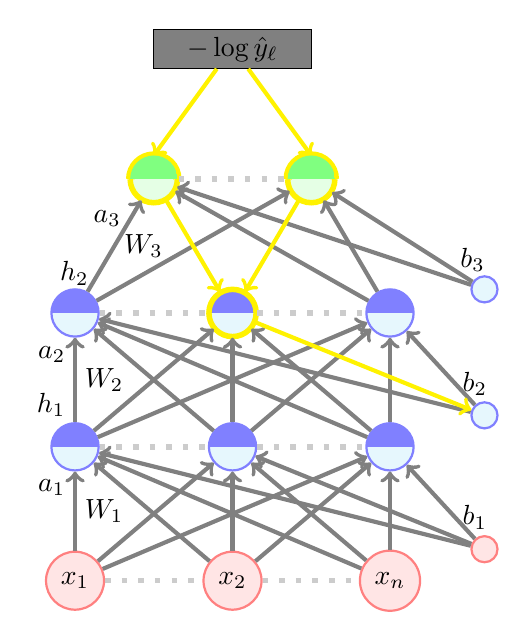
\begin{tikzpicture}
	\node [input_neuron] (neuron01) at (0,0) {$x_1$};
	\node [input_neuron] (neuron02) at (2,0){$x_2$};
	\node [input_neuron] (neuron03) at (4,0) {$x_n$};

	\node [bias_neuron] (neuron04) at (5.2,0.4) {};


	\node [hidden_neuron] (neuron11) at (0,1.7)  {};
	\node [hidden_neuron] (neuron12) at (2,1.7)  {};
	\node [hidden_neuron] (neuron13) at (4,1.7)  {};

	\node [bias_hidden_neuron] (neuron14) at (5.2,2.1) {};

	\begin{scope}
		\path[clip] (0,1.7) circle (3mm);
		\path[fill=blue!50] (-0.4,1.7) rectangle (0.3,2);
	\end{scope}
	\begin{scope}
		\path[clip] (2,1.7) circle (3mm);
		\path[fill=blue!50] (1.6,1.7) rectangle (2.3,2);
	\end{scope}
	\begin{scope}
		\path[clip] (4,1.7) circle (3mm);
		\path[fill=blue!50] (3.6,1.7) rectangle (4.3,2);
	\end{scope}


	\node [hidden_neuron] (neuron21) at (0,3.4)  {};
	\node [hidden_neuron] (neuron22) at (2,3.4)  {};
	\node [hidden_neuron] (neuron23) at (4,3.4)  {};

	\node [bias_hidden_neuron] (neuron24) at (5.2,3.7) {};


	\begin{scope}
		\path[clip] (0,3.4) circle (3mm);
		\path[fill=blue!50] (-0.4,3.4) rectangle (0.4,3.7);
	\end{scope}
	\begin{scope}
		\path[clip] (2,3.4) circle (3mm);
		\path[fill=blue!50] (1.6,3.4) rectangle (2.4,3.7);
	\end{scope}
	\begin{scope}
		\path[clip] (4,3.4) circle (3mm);
		\path[fill=blue!50] (3.6,3.4) rectangle (4.4,3.7);
	\end{scope}


	\node [output_neuron] (neuron31) at (1,5.1)  {};
	\node [output_neuron] (neuron32) at (3,5.1)  {};
	\draw [fill=gray] (1, 7) rectangle (3, 6.5) node[pos=0.5] {$-\log\hat{y}_\ell$};
	\draw [yellow,line width=1.5pt,  ->]   (1.8, 6.5) --(1,5.4);
	\draw [yellow, line width=1.5pt, ->]   (2.2, 6.5)-- (3,5.4);
	\draw[yellow, line width = 2] (1.7, 3.4) arc (180:360:3mm){};
	\draw [yellow, line width = 3] (1.3,5.1) arc (0:180:3mm) {};
	\draw [yellow, line width = 3] (3.3,5.1) arc (0:180:3mm) {};
	\draw[yellow, line width = 2] (0.7, 5.1) arc (180:360:3mm){};
	\draw[yellow, line width = 2] (2.7, 5.1) arc (180:360:3mm){};
	\draw[yellow, line width = 2] (2.3, 3.4) arc (0:180:3mm){};

	\begin{scope}
		\path[clip] (1,5.1) circle (3mm);
		\path[fill=green!50] (0.6,5.1) rectangle (1.3,5.4);
	\end{scope}
	\begin{scope}
		\path[clip] (3,5.1) circle (3mm);
		\path[fill=green!50] (2.6,5.1) rectangle (3.3,5.4);
	\end{scope}

	\draw[white,->] (neuron01) -- (neuron11) node[black,pos=.5,right]  {$W_{1}$} node[black,pos=0.8,left] {$a_{1}$};

	\draw[white,->] (neuron11) -- (neuron21) node[black,pos=.5,right] {$W_{2}$} node[black,pos=0.8,left] {$a_{2}$} node[black,pos=.2,left] {$h_{1}$};
	\draw[white,->] (neuron21) -- (neuron31) node[black,pos=.5,right] {$W_{3}$} node[black,pos=0.8,left] {$a_{3}$} node[black,pos=.2,left] {$h_{2}$};

	\draw[white,->] (neuron04) -- (neuron13) node[black,pos=0,right,above] {$b_1$};

	\draw[white,->] (neuron14) -- (neuron23) node[black,pos=0,right,above] {$b_2$};

	\draw[white,->] (neuron24) -- (neuron32) node[black,pos=0,right,above] {$b_3$};


	%\draw[white,->] (neuron31) -- (2.4.9) node[black,pos=1,above] {y };
	%\draw[white,->] (neuron31) -- (3,6.5) node[black,pos=1,above] {$f(x)$};
	%node[pos=1.3,above,right] {$\mathscr{L}(\theta)$};

	\draw[black!20,line width=2pt,loosely dotted] (neuron01) -- (neuron02);
	\draw[black!20,line width=2pt,loosely dotted] (neuron02) -- (neuron03);
	\draw[black!20,line width=2pt,loosely dotted] (neuron11) -- (neuron12);
	\draw[black!20,line width=2pt,loosely dotted] (neuron12) -- (neuron13);
	\draw[black!20,line width=2pt,loosely dotted] (neuron21) -- (neuron22);
	\draw[black!20,line width=2pt,loosely dotted] (neuron22) -- (neuron23);
	\draw[black!20,line width=2pt,loosely dotted] (neuron31) -- (neuron32);


	\foreach \from in {neuron01,neuron02,neuron03,neuron04}
	\foreach \to in {neuron11,neuron12,neuron13}
	\draw [black!50,line width=1.5pt,->] (\from) -- (\to);

	\foreach \from in {neuron11,neuron12,neuron13}
	\foreach \to in {neuron21,neuron23}
	\draw [black!50,line width=1.5pt,->] (\from) -- (\to);

	\foreach \from in {neuron21,neuron23, neuron24}
	\foreach \to in {neuron31,neuron32}
	\draw [black!50,line width=1.5pt,->] (\from) -- (\to);

	\draw [black!50, line width=1.5pt, ->] (neuron14)--(neuron21);
	\draw [black!50, line width=1.5pt, ->] (neuron14)--(neuron23);

	\draw [black!50, line width=1.5pt, ->] (neuron11)--(neuron22);
	\draw [black!50, line width=1.5pt, ->] (neuron12)--(neuron22);
	\draw [black!50, line width=1.5pt, ->] (neuron13)--(neuron22);

	\draw [yellow, line width=1.5pt, ->] (neuron22) -- (neuron14);
	\draw [yellow, line width=1.5pt, ->] (neuron31) -- (neuron22);
	\draw [yellow, line width=1.5pt, ->] (neuron32) -- (neuron22);

\end{tikzpicture}
}
\savestack{\nnweight}{\hspace{-0.1in}
\tikzstyle{input_neuron}=[circle,draw=red!50,fill=red!10,thick,minimum size=5mm]
\tikzstyle{hidden_neuron}=[circle,draw=blue!50,fill=cyan!10,thick,minimum size=6mm]
\tikzstyle{output_neuron}=[circle,draw=green!50,fill=green!10,thick,minimum size=6mm]
\tikzstyle{bias_neuron}=[circle,draw=red!50,fill=red!10,thick,minimum size=2mm]
\tikzstyle{bias_hidden_neuron}=[circle,draw=blue!50,fill=cyan!10,thick,minimum size=2mm]

\tikzstyle{input}=[circle,draw=black!50,fill=black!20,thick,minimum size=6mm]

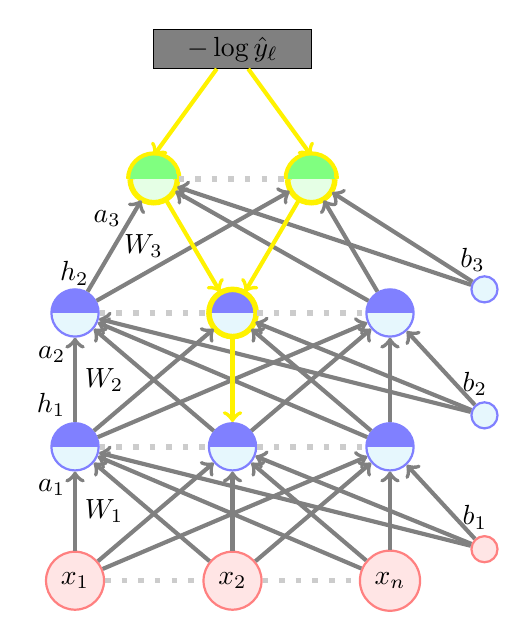
\begin{tikzpicture}
	\node [input_neuron] (neuron01) at (0,0) {$x_1$};
	\node [input_neuron] (neuron02) at (2,0){$x_2$};
	\node [input_neuron] (neuron03) at (4,0) {$x_n$};

	\node [bias_neuron] (neuron04) at (5.2,0.4) {};


	\node [hidden_neuron] (neuron11) at (0,1.7)  {};
	\node [hidden_neuron] (neuron12) at (2,1.7)  {};
	\node [hidden_neuron] (neuron13) at (4,1.7)  {};

	\node [bias_hidden_neuron] (neuron14) at (5.2,2.1) {};

	\begin{scope}
		\path[clip] (0,1.7) circle (3mm);
		\path[fill=blue!50] (-0.4,1.7) rectangle (0.3,2);
	\end{scope}
	\begin{scope}
		\path[clip] (2,1.7) circle (3mm);
		\path[fill=blue!50] (1.6,1.7) rectangle (2.3,2);
	\end{scope}
	\begin{scope}
		\path[clip] (4,1.7) circle (3mm);
		\path[fill=blue!50] (3.6,1.7) rectangle (4.3,2);
	\end{scope}


	\node [hidden_neuron] (neuron21) at (0,3.4)  {};
	\node [hidden_neuron] (neuron22) at (2,3.4)  {};
	\node [hidden_neuron] (neuron23) at (4,3.4)  {};

	\node [bias_hidden_neuron] (neuron24) at (5.2,3.7) {};


	\begin{scope}
		\path[clip] (0,3.4) circle (3mm);
		\path[fill=blue!50] (-0.4,3.4) rectangle (0.4,3.7);
	\end{scope}
	\begin{scope}
		\path[clip] (2,3.4) circle (3mm);
		\path[fill=blue!50] (1.6,3.4) rectangle (2.4,3.7);
	\end{scope}
	\begin{scope}
		\path[clip] (4,3.4) circle (3mm);
		\path[fill=blue!50] (3.6,3.4) rectangle (4.4,3.7);
	\end{scope}


	\node [output_neuron] (neuron31) at (1,5.1)  {};
	\node [output_neuron] (neuron32) at (3,5.1)  {};
	\draw [fill=gray] (1, 7) rectangle (3, 6.5) node[pos=0.5] {$-\log\hat{y}_\ell$};
	\draw [yellow,line width=1.5pt,  ->]   (1.8, 6.5) --(1,5.4);
	\draw [yellow, line width=1.5pt, ->]   (2.2, 6.5)-- (3,5.4);
	\draw[yellow, line width = 2] (1.7, 3.4) arc (180:360:3mm){};
	\draw [yellow, line width = 3] (1.3,5.1) arc (0:180:3mm) {};
	\draw [yellow, line width = 3] (3.3,5.1) arc (0:180:3mm) {};
	\draw[yellow, line width = 2] (0.7, 5.1) arc (180:360:3mm){};
	\draw[yellow, line width = 2] (2.7, 5.1) arc (180:360:3mm){};
	\draw[yellow, line width = 2] (2.3, 3.4) arc (0:180:3mm){};

	\begin{scope}
		\path[clip] (1,5.1) circle (3mm);
		\path[fill=green!50] (0.6,5.1) rectangle (1.3,5.4);
	\end{scope}
	\begin{scope}
		\path[clip] (3,5.1) circle (3mm);
		\path[fill=green!50] (2.6,5.1) rectangle (3.3,5.4);
	\end{scope}

	\draw[white,->] (neuron01) -- (neuron11) node[black,pos=.5,right]  {$W_{1}$} node[black,pos=0.8,left] {$a_{1}$};

	\draw[white,->] (neuron11) -- (neuron21) node[black,pos=.5,right] {$W_{2}$} node[black,pos=0.8,left] {$a_{2}$} node[black,pos=.2,left] {$h_{1}$};
	\draw[white,->] (neuron21) -- (neuron31) node[black,pos=.5,right] {$W_{3}$} node[black,pos=0.8,left] {$a_{3}$} node[black,pos=.2,left] {$h_{2}$};

	\draw[white,->] (neuron04) -- (neuron13) node[black,pos=0,right,above] {$b_1$};

	\draw[white,->] (neuron14) -- (neuron23) node[black,pos=0,right,above] {$b_2$};

	\draw[white,->] (neuron24) -- (neuron32) node[black,pos=0,right,above] {$b_3$};

	\draw[black!20,line width=2pt,loosely dotted] (neuron01) -- (neuron02);
	\draw[black!20,line width=2pt,loosely dotted] (neuron02) -- (neuron03);
	\draw[black!20,line width=2pt,loosely dotted] (neuron11) -- (neuron12);
	\draw[black!20,line width=2pt,loosely dotted] (neuron12) -- (neuron13);
	\draw[black!20,line width=2pt,loosely dotted] (neuron21) -- (neuron22);
	\draw[black!20,line width=2pt,loosely dotted] (neuron22) -- (neuron23);
	\draw[black!20,line width=2pt,loosely dotted] (neuron31) -- (neuron32);


	\foreach \from in {neuron01,neuron02,neuron03,neuron04}
	\foreach \to in {neuron11,neuron12,neuron13}
	\draw [black!50,line width=1.5pt,->] (\from) -- (\to);

	\foreach \from in {neuron11,neuron12,neuron13,neuron14}
	\foreach \to in {neuron21,neuron23}
	\draw [black!50,line width=1.5pt,->] (\from) -- (\to);

	\foreach \from in {neuron21,neuron23,neuron24}
	\foreach \to in {neuron31,neuron32}
	\draw [black!50,line width=1.5pt,->] (\from) -- (\to);

	\draw [black!50, line width=1.5pt, ->] (neuron11)--(neuron22);
	\draw [black!50, line width=1.5pt, ->] (neuron13)--(neuron22);
	\draw [black!50, line width=1.5pt, ->] (neuron14)--(neuron22);
	\draw [yellow, line width=1.5pt, ->] (neuron22) -- (neuron12);
	\draw [yellow, line width=1.5pt, ->] (neuron31) -- (neuron22);
	\draw [yellow, line width=1.5pt, ->] (neuron32) -- (neuron22);

\end{tikzpicture}
}

\begin{frame}
  \myheading{Module 4.7: Backpropagation: Computing Gradients w.r.t. Parameters}
\end{frame}

%Slide 36
\begin{frame}
  \begin{overlayarea}{\textwidth}{\textheight}
    \textbf{Quantities of interest (roadmap for the remaining part):}
    \begin{itemize}
      \justifying
      \item Gradient w.r.t. output units
      \item Gradient w.r.t. hidden units
      \item \alert<1->{Gradient w.r.t. weights and biases}
    \end{itemize}

    \begin{align*}
      \underbrace{\frac{\partial \mathscr{L}(\theta)}{\partial W_{111}}}_
      {\substack{\text{Talk to the}\\ \text{weight directly}}}
      =
      {\underbrace{\frac{\partial \mathscr{L}(\theta)}{\partial \hat{y}} \frac{\partial \hat{y}}{\partial a_{3}}}_
        {\substack{\text{Talk to the} \\ \text{output layer}}}} 
      {\underbrace{\frac{\partial a_{3}}{\partial h_{2}} \frac{\partial h_{2}}{\partial a_{2}}}_
        {\substack{\text{Talk to the} \\ \text{previous hidden} \\ \text{layer}}}
        \underbrace{\frac{\partial a_{2}}{\partial h_{1}} \frac{\partial h_{1}}{\partial a_{1}}}_
        {\substack{\text{Talk to the} \\ \text{previous} \\ \text{hidden layer}}}} 
      \alert<1->{\underbrace{\frac{\partial a_{1}}{\partial W_{111}}}_
        {\substack{\text{and now} \\ \text{talk to} \\ \text{the} \\ \text{weights}}}}
    \end{align*}

    \begin{itemize}
      \justifying
      \item<1-> Our focus is on \textit{Cross entropy loss} and \textit{Softmax} output.
    \end{itemize}
  \end{overlayarea}
\end{frame}

%Slide 37
\begin{frame}
  \begin{columns}
    \column{0.6\textwidth}
    \begin{overlayarea}{\textwidth}{\textheight}
      \justifying
      Recall that,
      \begin{align*}
        \mathbf{a_k}                                                                    & =  \mathbf{b_k}  + W_k \mathbf{h_{k-1}} \\
        % \visible<2->{a_{ki}                                                             & =  b_{ki} + W_{kij} h_{k-1,j} \\}
        \visible<2->{\frac{\partial a_{ki}}{\partial W_{kij}}                           & = h_{k-1,j} \\}
        \visible<3->{\frac{\partial\mathscr{L(\theta)}}{\partial W_{kij}} \visible<4->{ & = \frac{\partial\mathscr{L(\theta)}}{\partial a_{ki}} \frac{\partial a_{ki}}{\partial W_{k,i,j}}}\\}
        \visible<5->{                                                                   & =\frac{\partial\mathscr{L(\theta)}}{\partial a_{ki}} h_{k-1,j}\\}
        \visible<6->{\nabla_{W_K} \mathscr{L(\theta)}                                   & =} \visible<7->{\begin{bmatrix}
            \frac{\partial\mathscr{L(\theta)}}{\partial W_{k00}} &
            \frac{\partial\mathscr{L(\theta)}}{\partial W_{k01}}
            & \dots &\dots &   \frac{\partial\mathscr{L(\theta)}}{\partial W_{k0n-1}} \\
            \dots  & \dots  & \dots  & \dots  & \dots                                                      \\
            \vdots & \vdots & \vdots & \vdots & \vdots                                                     \\
            \dots  & \dots  & \dots  & \dots  & \frac{\partial\mathscr{L(\theta)}}{\partial W_{k,n-1,n-1}}
          \end{bmatrix}}
      \end{align*}
    \end{overlayarea}

    \column{0.4\textwidth}
    \begin{overlayarea}{\textwidth}{\textheight}
      \makebox[\textwidth][c]{\usebox{\nnweightcontent}}
    \end{overlayarea}
    % \hspace{-0.1in}
\tikzstyle{input_neuron}=[circle,draw=red!50,fill=red!10,thick,minimum size=5mm]
\tikzstyle{hidden_neuron}=[circle,draw=blue!50,fill=cyan!10,thick,minimum size=6mm]
\tikzstyle{output_neuron}=[circle,draw=green!50,fill=green!10,thick,minimum size=6mm]
\tikzstyle{bias_neuron}=[circle,draw=red!50,fill=red!10,thick,minimum size=2mm]
\tikzstyle{bias_hidden_neuron}=[circle,draw=blue!50,fill=cyan!10,thick,minimum size=2mm]

\tikzstyle{input}=[circle,draw=black!50,fill=black!20,thick,minimum size=6mm]

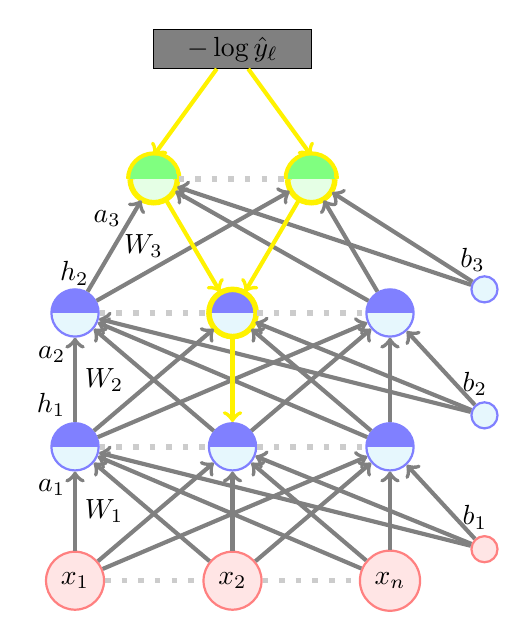
\begin{tikzpicture}
	\node [input_neuron] (neuron01) at (0,0) {$x_1$};
	\node [input_neuron] (neuron02) at (2,0){$x_2$};
	\node [input_neuron] (neuron03) at (4,0) {$x_n$};

	\node [bias_neuron] (neuron04) at (5.2,0.4) {};


	\node [hidden_neuron] (neuron11) at (0,1.7)  {};
	\node [hidden_neuron] (neuron12) at (2,1.7)  {};
	\node [hidden_neuron] (neuron13) at (4,1.7)  {};

	\node [bias_hidden_neuron] (neuron14) at (5.2,2.1) {};

	\begin{scope}
		\path[clip] (0,1.7) circle (3mm);
		\path[fill=blue!50] (-0.4,1.7) rectangle (0.3,2);
	\end{scope}
	\begin{scope}
		\path[clip] (2,1.7) circle (3mm);
		\path[fill=blue!50] (1.6,1.7) rectangle (2.3,2);
	\end{scope}
	\begin{scope}
		\path[clip] (4,1.7) circle (3mm);
		\path[fill=blue!50] (3.6,1.7) rectangle (4.3,2);
	\end{scope}


	\node [hidden_neuron] (neuron21) at (0,3.4)  {};
	\node [hidden_neuron] (neuron22) at (2,3.4)  {};
	\node [hidden_neuron] (neuron23) at (4,3.4)  {};

	\node [bias_hidden_neuron] (neuron24) at (5.2,3.7) {};


	\begin{scope}
		\path[clip] (0,3.4) circle (3mm);
		\path[fill=blue!50] (-0.4,3.4) rectangle (0.4,3.7);
	\end{scope}
	\begin{scope}
		\path[clip] (2,3.4) circle (3mm);
		\path[fill=blue!50] (1.6,3.4) rectangle (2.4,3.7);
	\end{scope}
	\begin{scope}
		\path[clip] (4,3.4) circle (3mm);
		\path[fill=blue!50] (3.6,3.4) rectangle (4.4,3.7);
	\end{scope}


	\node [output_neuron] (neuron31) at (1,5.1)  {};
	\node [output_neuron] (neuron32) at (3,5.1)  {};
	\draw [fill=gray] (1, 7) rectangle (3, 6.5) node[pos=0.5] {$-\log\hat{y}_\ell$};
	\draw [yellow,line width=1.5pt,  ->]   (1.8, 6.5) --(1,5.4);
	\draw [yellow, line width=1.5pt, ->]   (2.2, 6.5)-- (3,5.4);
	\draw[yellow, line width = 2] (1.7, 3.4) arc (180:360:3mm){};
	\draw [yellow, line width = 3] (1.3,5.1) arc (0:180:3mm) {};
	\draw [yellow, line width = 3] (3.3,5.1) arc (0:180:3mm) {};
	\draw[yellow, line width = 2] (0.7, 5.1) arc (180:360:3mm){};
	\draw[yellow, line width = 2] (2.7, 5.1) arc (180:360:3mm){};
	\draw[yellow, line width = 2] (2.3, 3.4) arc (0:180:3mm){};

	\begin{scope}
		\path[clip] (1,5.1) circle (3mm);
		\path[fill=green!50] (0.6,5.1) rectangle (1.3,5.4);
	\end{scope}
	\begin{scope}
		\path[clip] (3,5.1) circle (3mm);
		\path[fill=green!50] (2.6,5.1) rectangle (3.3,5.4);
	\end{scope}

	\draw[white,->] (neuron01) -- (neuron11) node[black,pos=.5,right]  {$W_{1}$} node[black,pos=0.8,left] {$a_{1}$};

	\draw[white,->] (neuron11) -- (neuron21) node[black,pos=.5,right] {$W_{2}$} node[black,pos=0.8,left] {$a_{2}$} node[black,pos=.2,left] {$h_{1}$};
	\draw[white,->] (neuron21) -- (neuron31) node[black,pos=.5,right] {$W_{3}$} node[black,pos=0.8,left] {$a_{3}$} node[black,pos=.2,left] {$h_{2}$};

	\draw[white,->] (neuron04) -- (neuron13) node[black,pos=0,right,above] {$b_1$};

	\draw[white,->] (neuron14) -- (neuron23) node[black,pos=0,right,above] {$b_2$};

	\draw[white,->] (neuron24) -- (neuron32) node[black,pos=0,right,above] {$b_3$};

	\draw[black!20,line width=2pt,loosely dotted] (neuron01) -- (neuron02);
	\draw[black!20,line width=2pt,loosely dotted] (neuron02) -- (neuron03);
	\draw[black!20,line width=2pt,loosely dotted] (neuron11) -- (neuron12);
	\draw[black!20,line width=2pt,loosely dotted] (neuron12) -- (neuron13);
	\draw[black!20,line width=2pt,loosely dotted] (neuron21) -- (neuron22);
	\draw[black!20,line width=2pt,loosely dotted] (neuron22) -- (neuron23);
	\draw[black!20,line width=2pt,loosely dotted] (neuron31) -- (neuron32);


	\foreach \from in {neuron01,neuron02,neuron03,neuron04}
	\foreach \to in {neuron11,neuron12,neuron13}
	\draw [black!50,line width=1.5pt,->] (\from) -- (\to);

	\foreach \from in {neuron11,neuron12,neuron13,neuron14}
	\foreach \to in {neuron21,neuron23}
	\draw [black!50,line width=1.5pt,->] (\from) -- (\to);

	\foreach \from in {neuron21,neuron23,neuron24}
	\foreach \to in {neuron31,neuron32}
	\draw [black!50,line width=1.5pt,->] (\from) -- (\to);

	\draw [black!50, line width=1.5pt, ->] (neuron11)--(neuron22);
	\draw [black!50, line width=1.5pt, ->] (neuron13)--(neuron22);
	\draw [black!50, line width=1.5pt, ->] (neuron14)--(neuron22);
	\draw [yellow, line width=1.5pt, ->] (neuron22) -- (neuron12);
	\draw [yellow, line width=1.5pt, ->] (neuron31) -- (neuron22);
	\draw [yellow, line width=1.5pt, ->] (neuron32) -- (neuron22);

\end{tikzpicture}

  \end{columns}
\end{frame}

\begin{frame}[b]
    \visible<1>{\tiny Intentionally left blank}
\end{frame}

%Slide 38
\begin{frame}
  \begin{overlayarea}{\textwidth}{\textheight}
    \visible<1->{Lets take a simple example of a $W_k \in \mathbb{R}^{3 \times 3}$ and see what each entry looks like}
    \\~\\
    \visible<2->{
      $\nabla_{W_k}\mathscr{L}(\theta)= \begin{bmatrix}
          \frac{\partial \mathscr{L}(\theta)}{\partial W_{k00}} & \frac{\partial \mathscr{L}(\theta)}{\partial W_{k01}} & \frac{\partial \mathscr{L}(\theta)}{\partial W_{k02}} \\
          & & \\
          \frac{\partial \mathscr{L}(\theta)}{\partial W_{k10}} & \frac{\partial \mathscr{L}(\theta)}{\partial W_{k11}} & \frac{\partial \mathscr{L}(\theta)}{\partial W_{k12}} \\
          & & \\
          \frac{\partial \mathscr{L}(\theta)}{\partial W_{k20}} & \frac{\partial \mathscr{L}(\theta)}{\partial W_{k21}} & \frac{\partial \mathscr{L}(\theta)}{\partial W_{k22}} \\
        \end{bmatrix} \frac{\partial\mathscr{L(\theta)}}{\partial W_{kij}} \visible<2->{= \frac{\partial\mathscr{L(\theta)}}{\partial a_{ki}} \frac{\partial a_{ki}}{\partial W_{k,i,j}}}$
    }
    \vspace{1cm}
    \visible<3->{
      $ \nabla_{W_k}\mathscr{L}(\theta) = \begin{bmatrix}
          \color<7->{brown} {\frac{\partial \mathscr{L}(\theta)} {\partial a_{k0}}} \color{black} \color<4->{blue}{h_{k-1,0}} \color{black}  & \color<7->{brown} {\frac{\partial \mathscr{L}(\theta)}{\partial a_{k0}}}  \color{black} \color<5->{red}{h_{k-1,1}} \color{black}  & \color<7->{brown} {\frac{\partial \mathscr{L}(\theta)}{\partial a_{k0}}} \color{black} \color<6->{orange}{h_{k-1,2}} \color{black}  \\
          & & \\
          \color<7->{magenta} {\frac{\partial \mathscr{L}(\theta)}{\partial a_{k1}}} \color{black} \color<4->{blue}{h_{k-1,0}} \color{black} & \color<7->{magenta} {\frac{\partial \mathscr{L}(\theta)}{\partial a_{k1}}} \color{black} \color<5->{red}{h_{k-1,1}} \color{black} & \color<7->{magenta} {\frac{\partial \mathscr{L}(\theta)}{\partial a_{k1}}} \color{black}\color<6->{orange}{h_{k-1,2}} \color{black} \\
           & & \\
          \frac{\partial \mathscr{L}(\theta)}{\partial a_{k2}} \color{black} \color<4->{blue}{h_{k-1,0}}  \color{black}                      & \frac{\partial \mathscr{L}(\theta)}{\partial a_{k2}} \color{black} \color<5->{red}{h_{k-1,1}} \color{black}                       & \frac{\partial \mathscr{L}(\theta)}{\partial a_{k2}} \color{black} \color<6->{orange}{h_{k-1,2}} \color{black}                      \\
        \end{bmatrix} = \visible<8->{\nabla_{a_k} \mathscr{L}(\theta) \cdot \mathbf{h_{k-1}}  ^T}$
    }

  \end{overlayarea}
\end{frame}

%Slide 39
\begin{frame}
  \begin{columns}
    \column{0.6\textwidth}
    \begin{overlayarea}{\textwidth}{\textheight}
      Finally, coming to the biases
        \begin{align*}
          \visible<2->{a_{ki}                                                & =  b_{ki} + \sum_j W_{kij} h_{k-1,j} \\}
          \visible<3->{\frac{\partial \mathscr{L}(\theta)} {\partial b_{ki}} & = \frac{\partial \mathscr{L}(\theta)}{\partial a_{ki}} \frac{\partial a_{ki}} {\partial b_{ki}} \\}
          \visible<4->{                                                      & = \frac{\partial \mathscr{L}(\theta)}{\partial {a_{ki}}}}
        \end{align*}
          \visible<5->{We can now write the gradient w.r.t. the vector $b_k$}
        \begin{align*}
          \visible<6->{\nabla_\mathbf{b_k}\mathscr{L}(\theta)                       & =
            \begin{bmatrix}
              \frac{\partial \mathscr{L}(\theta)}{a_{k_0}} \\
              \frac{\partial \mathscr{L}(\theta)}{a_{k_1}} \\
              \vdots                                       \\
              \frac{\partial \mathscr{L}(\theta)}{a_{k_n}}
            \end{bmatrix}}
          \visible<7->{= \nabla_{{\mathbf{a_k}}}\mathscr{L}(\theta)}
        \end{align*}
    \end{overlayarea}

    \column{0.4\textwidth}
    \begin{overlayarea}{\textwidth}{\textheight}
      \makebox[\textwidth][c]{\usebox{\nnbiascontent}}
    \end{overlayarea}
    % \hspace{-0.1in}
\tikzstyle{input_neuron}=[circle,draw=red!50,fill=red!10,thick,minimum size=5mm]
\tikzstyle{hidden_neuron}=[circle,draw=blue!50,fill=cyan!10,thick,minimum size=6mm]
\tikzstyle{output_neuron}=[circle,draw=green!50,fill=green!10,thick,minimum size=6mm]
\tikzstyle{bias_neuron}=[circle,draw=red!50,fill=red!10,thick,minimum size=2mm]
\tikzstyle{bias_hidden_neuron}=[circle,draw=blue!50,fill=cyan!10,thick,minimum size=2mm]

\tikzstyle{input}=[circle,draw=black!50,fill=black!20,thick,minimum size=6mm]

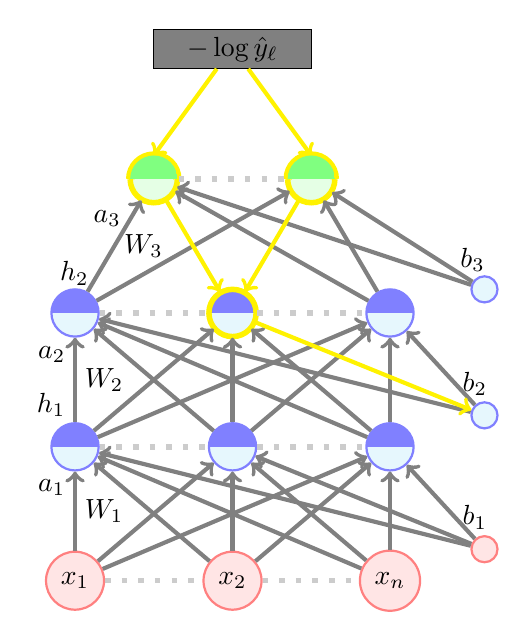
\begin{tikzpicture}
	\node [input_neuron] (neuron01) at (0,0) {$x_1$};
	\node [input_neuron] (neuron02) at (2,0){$x_2$};
	\node [input_neuron] (neuron03) at (4,0) {$x_n$};

	\node [bias_neuron] (neuron04) at (5.2,0.4) {};


	\node [hidden_neuron] (neuron11) at (0,1.7)  {};
	\node [hidden_neuron] (neuron12) at (2,1.7)  {};
	\node [hidden_neuron] (neuron13) at (4,1.7)  {};

	\node [bias_hidden_neuron] (neuron14) at (5.2,2.1) {};

	\begin{scope}
		\path[clip] (0,1.7) circle (3mm);
		\path[fill=blue!50] (-0.4,1.7) rectangle (0.3,2);
	\end{scope}
	\begin{scope}
		\path[clip] (2,1.7) circle (3mm);
		\path[fill=blue!50] (1.6,1.7) rectangle (2.3,2);
	\end{scope}
	\begin{scope}
		\path[clip] (4,1.7) circle (3mm);
		\path[fill=blue!50] (3.6,1.7) rectangle (4.3,2);
	\end{scope}


	\node [hidden_neuron] (neuron21) at (0,3.4)  {};
	\node [hidden_neuron] (neuron22) at (2,3.4)  {};
	\node [hidden_neuron] (neuron23) at (4,3.4)  {};

	\node [bias_hidden_neuron] (neuron24) at (5.2,3.7) {};


	\begin{scope}
		\path[clip] (0,3.4) circle (3mm);
		\path[fill=blue!50] (-0.4,3.4) rectangle (0.4,3.7);
	\end{scope}
	\begin{scope}
		\path[clip] (2,3.4) circle (3mm);
		\path[fill=blue!50] (1.6,3.4) rectangle (2.4,3.7);
	\end{scope}
	\begin{scope}
		\path[clip] (4,3.4) circle (3mm);
		\path[fill=blue!50] (3.6,3.4) rectangle (4.4,3.7);
	\end{scope}


	\node [output_neuron] (neuron31) at (1,5.1)  {};
	\node [output_neuron] (neuron32) at (3,5.1)  {};
	\draw [fill=gray] (1, 7) rectangle (3, 6.5) node[pos=0.5] {$-\log\hat{y}_\ell$};
	\draw [yellow,line width=1.5pt,  ->]   (1.8, 6.5) --(1,5.4);
	\draw [yellow, line width=1.5pt, ->]   (2.2, 6.5)-- (3,5.4);
	\draw[yellow, line width = 2] (1.7, 3.4) arc (180:360:3mm){};
	\draw [yellow, line width = 3] (1.3,5.1) arc (0:180:3mm) {};
	\draw [yellow, line width = 3] (3.3,5.1) arc (0:180:3mm) {};
	\draw[yellow, line width = 2] (0.7, 5.1) arc (180:360:3mm){};
	\draw[yellow, line width = 2] (2.7, 5.1) arc (180:360:3mm){};
	\draw[yellow, line width = 2] (2.3, 3.4) arc (0:180:3mm){};

	\begin{scope}
		\path[clip] (1,5.1) circle (3mm);
		\path[fill=green!50] (0.6,5.1) rectangle (1.3,5.4);
	\end{scope}
	\begin{scope}
		\path[clip] (3,5.1) circle (3mm);
		\path[fill=green!50] (2.6,5.1) rectangle (3.3,5.4);
	\end{scope}

	\draw[white,->] (neuron01) -- (neuron11) node[black,pos=.5,right]  {$W_{1}$} node[black,pos=0.8,left] {$a_{1}$};

	\draw[white,->] (neuron11) -- (neuron21) node[black,pos=.5,right] {$W_{2}$} node[black,pos=0.8,left] {$a_{2}$} node[black,pos=.2,left] {$h_{1}$};
	\draw[white,->] (neuron21) -- (neuron31) node[black,pos=.5,right] {$W_{3}$} node[black,pos=0.8,left] {$a_{3}$} node[black,pos=.2,left] {$h_{2}$};

	\draw[white,->] (neuron04) -- (neuron13) node[black,pos=0,right,above] {$b_1$};

	\draw[white,->] (neuron14) -- (neuron23) node[black,pos=0,right,above] {$b_2$};

	\draw[white,->] (neuron24) -- (neuron32) node[black,pos=0,right,above] {$b_3$};


	%\draw[white,->] (neuron31) -- (2.4.9) node[black,pos=1,above] {y };
	%\draw[white,->] (neuron31) -- (3,6.5) node[black,pos=1,above] {$f(x)$};
	%node[pos=1.3,above,right] {$\mathscr{L}(\theta)$};

	\draw[black!20,line width=2pt,loosely dotted] (neuron01) -- (neuron02);
	\draw[black!20,line width=2pt,loosely dotted] (neuron02) -- (neuron03);
	\draw[black!20,line width=2pt,loosely dotted] (neuron11) -- (neuron12);
	\draw[black!20,line width=2pt,loosely dotted] (neuron12) -- (neuron13);
	\draw[black!20,line width=2pt,loosely dotted] (neuron21) -- (neuron22);
	\draw[black!20,line width=2pt,loosely dotted] (neuron22) -- (neuron23);
	\draw[black!20,line width=2pt,loosely dotted] (neuron31) -- (neuron32);


	\foreach \from in {neuron01,neuron02,neuron03,neuron04}
	\foreach \to in {neuron11,neuron12,neuron13}
	\draw [black!50,line width=1.5pt,->] (\from) -- (\to);

	\foreach \from in {neuron11,neuron12,neuron13}
	\foreach \to in {neuron21,neuron23}
	\draw [black!50,line width=1.5pt,->] (\from) -- (\to);

	\foreach \from in {neuron21,neuron23, neuron24}
	\foreach \to in {neuron31,neuron32}
	\draw [black!50,line width=1.5pt,->] (\from) -- (\to);

	\draw [black!50, line width=1.5pt, ->] (neuron14)--(neuron21);
	\draw [black!50, line width=1.5pt, ->] (neuron14)--(neuron23);

	\draw [black!50, line width=1.5pt, ->] (neuron11)--(neuron22);
	\draw [black!50, line width=1.5pt, ->] (neuron12)--(neuron22);
	\draw [black!50, line width=1.5pt, ->] (neuron13)--(neuron22);

	\draw [yellow, line width=1.5pt, ->] (neuron22) -- (neuron14);
	\draw [yellow, line width=1.5pt, ->] (neuron31) -- (neuron22);
	\draw [yellow, line width=1.5pt, ->] (neuron32) -- (neuron22);

\end{tikzpicture}

  \end{columns}
\end{frame}